%=============================================================================
%  Rapport hebdomadaire de stage -- Semaine 6
%  Projet : Simulateur de controleur aerien -- copilote IA pour le controle aerien
%  Auteur : Nicolas Marano -- URCA / supercalculateur ROMEO (NVIDIA GH200)
%  Compilation : pdflatex (x2 pour la table des matieres)
%=============================================================================
\documentclass[11pt,a4paper]{article}

\usepackage[utf8]{inputenc}
\usepackage[T1]{fontenc}
\usepackage[french]{babel}
\usepackage{lmodern}
\usepackage{microtype}
\usepackage[a4paper,margin=2.3cm,headheight=15pt]{geometry}
\usepackage{graphicx}
\usepackage{booktabs}
\usepackage{array}
\usepackage[table]{xcolor}
\usepackage{titlesec}
\usepackage{enumitem}
\usepackage{caption}
\usepackage{fancyhdr}
\usepackage{listings}
\usepackage[most]{tcolorbox}
\usepackage{hyperref}

%--- Couleurs ----------------------------------------------------------------
\definecolor{atcblue}{RGB}{11,61,145}
\definecolor{atcteal}{RGB}{13,110,124}
\definecolor{atcgreen}{RGB}{22,128,71}
\definecolor{atcred}{RGB}{197,32,38}
\definecolor{atcpurple}{RGB}{109,40,180}
\definecolor{atcslate}{RGB}{71,85,105}
\definecolor{lightgray}{RGB}{244,246,249}
\definecolor{rulegray}{RGB}{210,216,224}

\hypersetup{colorlinks=true, linkcolor=atcblue, urlcolor=atcteal, citecolor=atcblue,
  pdftitle={Rapport de stage -- Semaine 6}, pdfauthor={Nicolas Marano}}

%--- Titres ------------------------------------------------------------------
\titleformat{\section}{\Large\bfseries\color{atcblue}}{\thesection}{0.6em}{}
\titleformat{\subsection}{\large\bfseries\color{atcteal}}{\thesubsection}{0.6em}{}
\titleformat{\subsubsection}{\normalsize\bfseries\color{atcteal}}{\thesubsubsection}{0.5em}{}
\titlespacing*{\section}{0pt}{16pt}{8pt}

%--- En-tete / pied de page --------------------------------------------------
\pagestyle{fancy}
\fancyhf{}
\renewcommand{\headrulewidth}{0.4pt}
\renewcommand{\footrulewidth}{0.4pt}
\fancyhead[L]{\small\color{atcblue}\itshape Copilote IA pour le controle aerien}
\fancyhead[R]{\small\color{atcblue}\itshape Semaine 6}
\fancyfoot[L]{\small Nicolas Marano, URCA / ROMEO}
\fancyfoot[R]{\small\thepage}

%--- Boites tcolorbox --------------------------------------------------------
\newtcolorbox{objbox}{enhanced, colback=lightgray, colframe=atcblue,
  boxrule=0.8pt, arc=3pt, left=10pt, right=10pt, top=8pt, bottom=8pt,
  fonttitle=\bfseries\color{white}, coltitle=white, colbacktitle=atcblue,
  title={Objectif de la semaine}}

\newtcolorbox{resbox}{enhanced, colback=atcgreen!6, colframe=atcgreen,
  boxrule=0.8pt, arc=3pt, left=10pt, right=10pt, top=8pt, bottom=8pt,
  fonttitle=\bfseries, coltitle=white, colbacktitle=atcgreen,
  title={Resultats cles}}

\newtcolorbox{warnbox}{enhanced, colback=atcslate!6, colframe=atcslate,
  boxrule=0.8pt, arc=3pt, left=10pt, right=10pt, top=8pt, bottom=8pt,
  fonttitle=\bfseries, coltitle=white, colbacktitle=atcslate,
  title={Contraintes techniques et choix d'ingenierie}}

%--- Style des listings ------------------------------------------------------
\lstdefinestyle{atccode}{
  basicstyle=\ttfamily\footnotesize,
  backgroundcolor=\color{lightgray},
  frame=single, framesep=5pt, rulecolor=\color{rulegray},
  breaklines=true, breakatwhitespace=true,
  showstringspaces=false,
  keywordstyle=\color{atcblue}\bfseries,
  commentstyle=\color{atcgreen}\itshape,
  stringstyle=\color{atcpurple},
  numberstyle=\tiny\color{gray},
  columns=fullflexible, keepspaces=true,
  aboveskip=8pt, belowskip=8pt,
}
\lstset{style=atccode}

\setlist[itemize]{label=\textbullet, leftmargin=1.4em, itemsep=2pt, topsep=3pt}
\captionsetup{font=small, labelfont={bf,color=atcblue}}
\renewcommand{\arraystretch}{1.25}

%=============================================================================
\begin{document}

%--- Page de garde -----------------------------------------------------------
\begin{titlepage}
\centering
\vspace*{1.2cm}
{\color{atcblue}\rule{\textwidth}{2pt}}\\[0.5cm]
{\Huge\bfseries\color{atcblue} Rapport d'avancement de stage\par}
\vspace{0.35cm}
{\LARGE\color{atcteal} Semaine 6\par}
\vspace{0.25cm}
{\large Synthese vocale par clonage de voix (XTTS) \\[2pt]
pour la generation a la volee de l'audio des pilotes virtuels\par}
\vspace{0.4cm}
{\color{atcblue}\rule{\textwidth}{2pt}}\\[1.0cm]

{\large\itshape Un copilote d'intelligence artificielle pour le controle aerien\par}
\vspace{1.6cm}

\begin{tabular}{rl}
\large\bfseries Auteur & \large Nicolas Marano\\[4pt]
\large\bfseries Projet & \large Simulateur de controleur aerien (PoC, 10 semaines)\\[4pt]
\large\bfseries Etablissement & \large Universite de Reims Champagne-Ardenne (URCA)\\[4pt]
\large\bfseries Calcul (IA) & \large Supercalculateur ROMEO : NVIDIA GH200 (Grace-Hopper, aarch64)\\[4pt]
\large\bfseries Domaine & \large Intelligence artificielle \& controle du trafic aerien\\[4pt]
\large\bfseries Periode & \large Semaine 6 du stage\\
\end{tabular}

\vfill
\begin{tcolorbox}[colback=lightgray, colframe=atcblue, arc=3pt, width=0.92\textwidth, center,
  left=12pt, right=12pt, top=8pt, bottom=8pt]
\small\centering
\textbf{Resume.} Cette semaine porte sur le module de synthese vocale, qui ferme la
boucle de dialogue en restituant la reponse du pilote en audio. La solution retenue
est un clonage de voix \emph{zero-shot} fonde sur le modele XTTS-v2 : a partir d'un
court extrait de reference, le systeme genere a la volee une voix distincte pour
chaque pilote virtuel, puis applique une degradation VHF (filtre de Butterworth
300--3400~Hz) pour reproduire le canal radio. La synthese est mesuree a 3,9~s par
collationnement (facteur temps reel 0,82, CPU) ; le taux d'erreur mots de
re-transcription de la voix synthetisee est de 22 a 24~\%.
\end{tcolorbox}
\vspace{0.6cm}
{\small Annee universitaire 2025--2026}
\end{titlepage}

%--- Table des matieres ------------------------------------------------------
\tableofcontents
\thispagestyle{fancy}
\vspace{1cm}

%=============================================================================
\section{Contexte et positionnement de la semaine}
%=============================================================================

Le projet automatise le dialogue radio pilote~/~controleur a l'interieur d'un
simulateur de trafic aerien. Une instruction parlee est transcrite, ancree dans la
phraseologie OACI, transformee en une commande validee, executee dans le simulateur
BlueSky, puis restituee sous forme d'un \emph{readback} (collationnement) en voix de
pilote synthetisee. La chaine cible se resume ainsi :

\begin{center}
\fbox{\parbox{0.95\textwidth}{\centering\ttfamily\footnotesize
voix pilote (VHF) $\rightarrow$ Whisper STT $\rightarrow$ NER + LLM avec RAG (OACI Doc 4444)
$\rightarrow$ JSON valide\\
$\rightarrow$ simulateur BlueSky (manoeuvre avion) $\rightarrow$ voix de readback synthetisee $\rightarrow$ boucle}}
\end{center}

Les semaines precedentes ont produit le module de \textbf{perception} (semaine~4,
reconnaissance vocale par Whisper fine-tune) et le module d'\textbf{interpretation}
(semaine~5, LLM ancre par RAG produisant un JSON valide et borne par une validation
de securite). La semaine~6 traite du \textbf{dernier maillon de la boucle} : la
\textbf{restitution vocale}. Il s'agit de convertir le texte du collationnement en
un signal audio credible, propre a chaque aeronef, afin que le simulateur ne se
contente pas d'executer la manoeuvre mais reponde egalement sur la frequence comme
le ferait un pilote reel.

\subsection{Synthese chiffree de la semaine}

\begin{table}[h]
\centering
\small
\begin{tabular}{>{\raggedright}p{8.7cm} l}
\toprule
\rowcolor{lightgray}\textbf{Indicateur} & \textbf{Resultat}\\
\midrule
Latence de synthese (par collationnement, CPU) & \textbf{3,9~s} (facteur temps reel 0,82)\\
WER de re-transcription de la voix synthetisee (S6/S8) & \textbf{22 a 24~\%}\\
WER de reference sur voix humaine reelle (validation S4) & 6,7~\%\\
Voix de reference clonees (pilotes / controleur distincts) & 3\\
Bande passante de degradation VHF (Butterworth ordre 6) & 300--3400~Hz\\
Boucle vocale complete rejouee et verifiee & oui (2026-06-11)\\
\bottomrule
\end{tabular}
\caption{Vue d'ensemble des resultats obtenus durant la semaine 6.}
\end{table}

%=============================================================================
\section{Semaine 6 : Synthese vocale par clonage de voix}
%=============================================================================

\begin{objbox}
Implementer une solution de \textbf{clonage vocal} permettant de generer a la volee
l'audio des differents pilotes virtuels. Chaque aeronef doit pouvoir prononcer son
collationnement avec une voix qui lui est propre, sans entrainement specifique par
locuteur, et dans un rendu sonore compatible avec le canal radio VHF du simulateur.
\end{objbox}

\subsection{Methode : clonage \emph{zero-shot} avec XTTS-v2}

La generation repose sur le modele \texttt{XTTS-v2} (paquet \texttt{coqui-tts}). Le
choix d'un clonage \emph{zero-shot} evite tout entrainement par locuteur : le modele
reproduit le timbre d'une voix a partir d'un seul extrait de reference de quelques
secondes, fourni au moment de la synthese. Cette approche permet d'attribuer une
voix distincte a chaque aeronef sans constituer de corpus dedie ni lancer de
campagne d'entrainement supplementaire, ce qui est adapte a la contrainte de calcul
et de stockage du cluster.

\begin{table}[h]
\centering
\small
\begin{tabular}{>{\raggedright}p{4.3cm} >{\raggedright}p{4.3cm} p{5.0cm}}
\toprule
\rowcolor{lightgray}\textbf{Composant} & \textbf{Valeur} & \textbf{Remarque}\\
\midrule
Modele & \texttt{XTTS-v2} (\texttt{coqui-tts}) & multilingue, clonage zero-shot\\
Strategie & clonage sans entrainement & voix clonee depuis un extrait de reference\\
Voix de reference & 3 extraits ATCO2 (4 a 9~s) & une voix par pilote virtuel\\
Frequence native & 24~kHz $\rightarrow$ 16~kHz & rééchantillonnage vers l'entree ASR\\
Langue & \texttt{en} & phraseologie anglaise\\
Materiel d'inference & CPU (noeud GH200) & contournement du bug cuFFT (GPU)\\
Post-traitement & degradation VHF 300--3400~Hz & rendu radio (\emph{sim-to-real})\\
\bottomrule
\end{tabular}
\caption{Configuration de la synthese vocale (semaine 6).}
\end{table}

\subsection{Chaine de synthese}

La fonction \texttt{synth()} enchaine quatre etapes deterministes apres la generation
XTTS : rééchantillonnage de 24~kHz vers 16~kHz (frequence d'entree du pipeline ASR),
normalisation d'amplitude pour eviter l'ecretage, puis degradation VHF. La sortie est
un signal mono 16~kHz directement consommable par le reste de la chaine.

\begin{center}
\fbox{\parbox{0.95\textwidth}{\centering\ttfamily\footnotesize
texte de readback (OACI) $\rightarrow$ XTTS-v2 (clonage, voix de reference)
$\rightarrow$ rééchantillonnage 24$\rightarrow$16 kHz\\
$\rightarrow$ normalisation $\rightarrow$ degradation VHF (Butterworth 300-3400 Hz)
$\rightarrow$ wav 16 kHz}}
\end{center}

\begin{lstlisting}[language=Python, caption={Coeur de la synthese : clonage XTTS puis post-traitement (extrait de \texttt{tts\_atc.py}).}]
wav = np.asarray(tts.tts(text=text, speaker_wav=ref_wav, language=language), dtype=np.float32)
wav16 = resample_poly(wav, FS, XTTS_SR).astype(np.float32)   # 24k -> 16k
peak = np.max(np.abs(wav16)) + 1e-9
if peak > 1.0:
    wav16 = wav16 / peak
if vhf:
    wav16 = preprocess_waveform(wav16, training=False)        # bande passante VHF 300-3400 Hz
\end{lstlisting}

\subsection{Generation du collationnement (phraseologie OACI)}

Le texte prononce n'est pas l'instruction brute mais un \emph{collationnement}
conforme a la phraseologie. Le module \texttt{readback.py} convertit les ordres JSON
en telephonie standard : chiffres epeles un a un (\texttt{niner} pour 9), indicatifs
en code telephonique (\texttt{AFR}~$\rightarrow$~\emph{air france}), points de
cheminement en alphabet OACI. Le sens d'un changement d'altitude (montee ou descente)
est determine en comparant la valeur cible a l'altitude courante de l'aeronef.

\begin{lstlisting}[caption={Exemple de collationnement genere a partir d'un ordre JSON.}]
Ordre : {callsign: AFR1234, action: ALT, value: 10000}  (avion au FL130)
Texte : "descend flight level one zero zero, air france one two three four"
\end{lstlisting}

\subsection{Voix de reference}

Les voix de reference sont extraites du corpus ATCO2 (jeu de test) par le module
\texttt{make\_pilot\_voices.py} : il selectionne trois segments courts (4 a 9~s,
non silencieux) qui servent de timbres a cloner. Chaque aeronef de la flotte se voit
attribuer une de ces voix, de sorte que des pilotes differents sonnent
differemment sur la frequence. L'usage d'extraits radio reels comme reference
contribue au realisme du rendu.

\subsection{Degradation VHF et coherence de domaine}

La voix synthetisee par XTTS est propre (large bande). Pour la rendre credible sur
une frequence aeronautique, la chaine applique la degradation VHF deja validee en
semaine~2 : un filtre passe-bande de Butterworth d'ordre~6, limite a la bande
300--3400~Hz (figure~\ref{fig:bode}). Cette etape a un second interet, au-dela du
realisme : elle place la voix synthetisee dans le \emph{meme domaine acoustique} que
les donnees sur lesquelles le module de reconnaissance vocale a ete specialise. La
re-transcription du collationnement reste ainsi coherente avec le reste de la chaine
(reduction du fosse \emph{sim-to-real}). La figure~\ref{fig:spectro} illustre l'effet
de ce filtrage sur un signal de parole.

\begin{figure}[h]
\centering
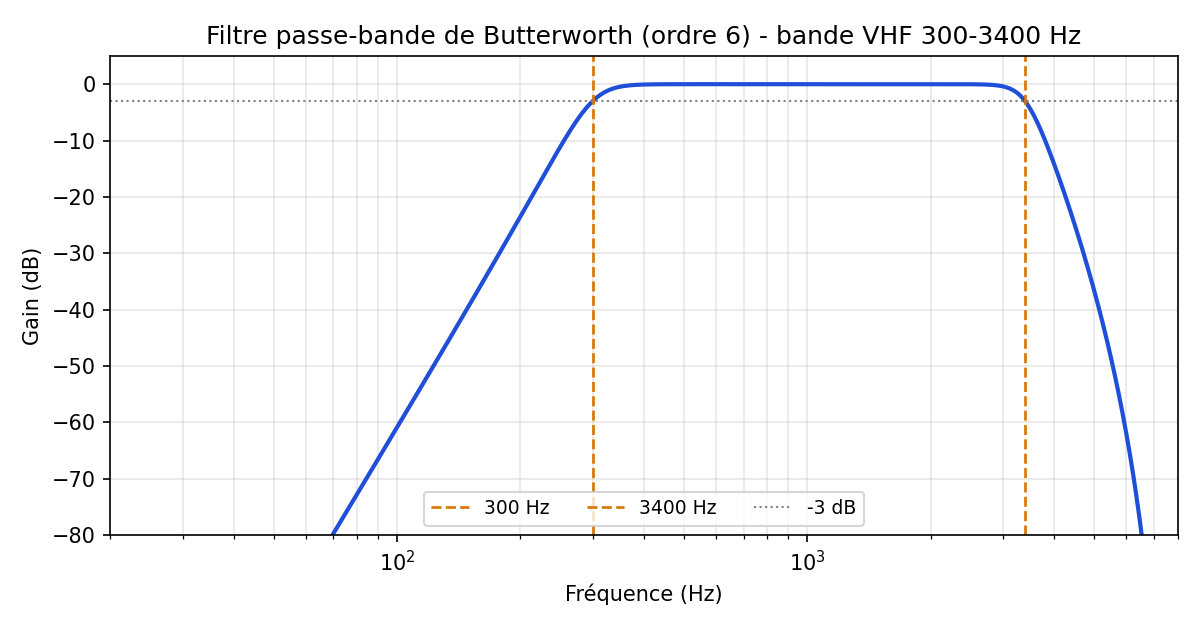
\includegraphics[width=0.72\textwidth]{figures/fig_butterworth_bode.png}
\caption{Reponse en frequence du filtre passe-bande de Butterworth (ordre~6) utilise
pour la degradation VHF. La bande utile est limitee a 300--3400~Hz, comme une radio
aeronautique.}
\label{fig:bode}
\end{figure}

\begin{figure}[h]
\centering
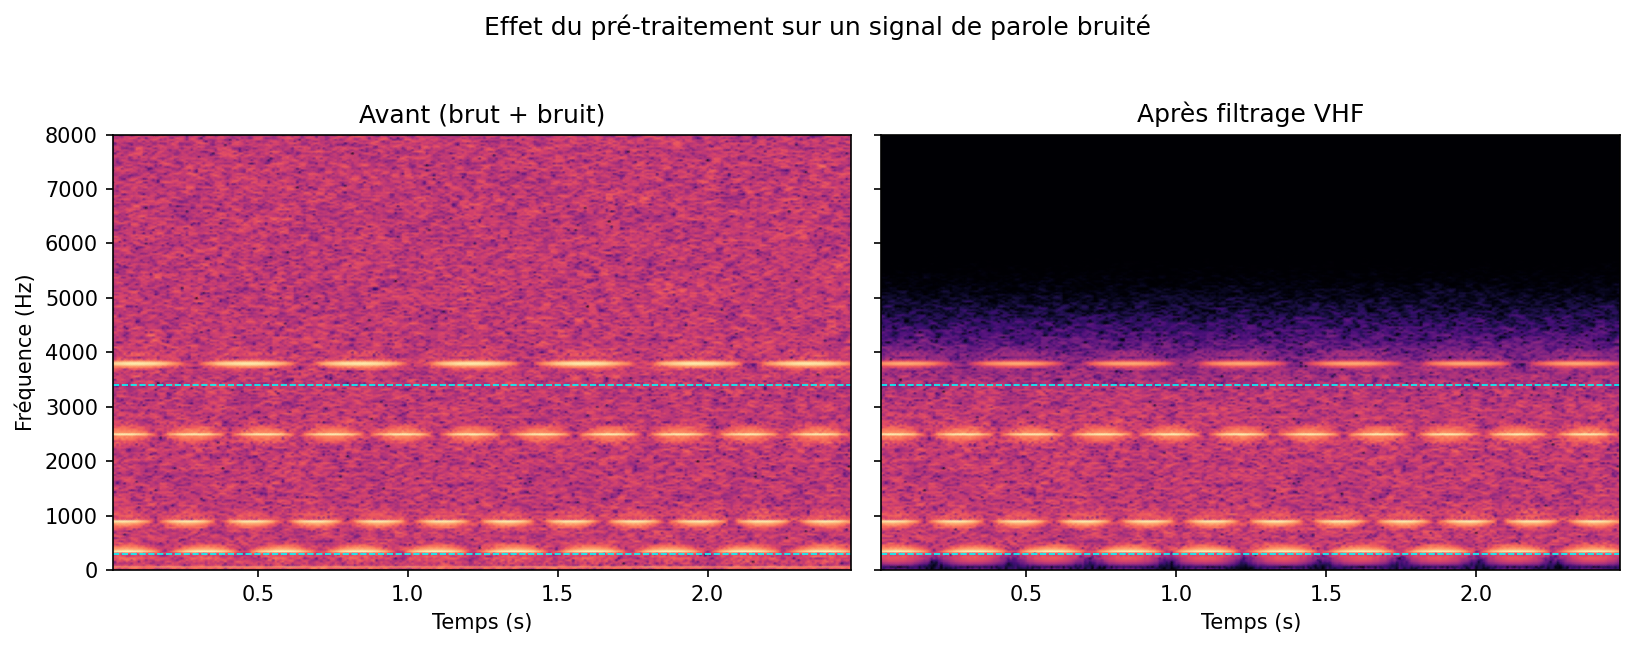
\includegraphics[width=0.86\textwidth]{figures/fig_spectrogramme_avant_apres.png}
\caption{Effet de la degradation VHF sur un signal de parole : spectre avant
(gauche) et apres filtrage passe-bande (droite). Le contenu hors bande 300--3400~Hz
est attenue, reproduisant la coloration d'un canal radio. La meme chaine est
appliquee a la voix synthetisee.}
\label{fig:spectro}
\end{figure}

\begin{warnbox}
L'integration de XTTS dans l'environnement logiciel du cluster a necessite plusieurs
ajustements. Le paquet \texttt{coqui-tts} a ete ajoute a l'environnement existant
(\emph{whisper-atc}) plutot que dans un environnement separe, afin de reutiliser la
meme version de PyTorch et de \texttt{transformers} : ce choix evite une seconde
installation de PyTorch, tient dans le quota disque de 20~Go et permet de servir les
trois modeles (Whisper, Mistral, XTTS) depuis un unique processus. Comme XTTS
importe un symbole (\texttt{isin\_mps\_friendly}) supprime dans \texttt{transformers}
5.x, ce symbole est restaure par un correctif applique avant l'import de la
bibliotheque, sans retrograder \texttt{transformers} (qui doit rester en version~5.9
pour Whisper et Mistral). Enfin, l'encodeur de locuteur de XTTS declenche un bug
cuFFT de \texttt{torchaudio} sur le GPU GH200 ; la synthese est donc executee sur
CPU, ce qui la rend fiable mais non temps reel.
\end{warnbox}

\subsection{Integration : la boucle vocale complete}

L'assemblage est valide par le module \texttt{voice\_exchange.py}, qui rejoue un
echange radio complet. Pour chaque instruction, le controleur parle (synthese~+~VHF),
l'audio est transcrit puis interprete, BlueSky execute l'ordre, et l'aeronef
collationne dans \emph{sa} voix clonee (synthese~+~VHF). Le collationnement est
ensuite re-transcrit pour verifier son intelligibilite, et les signaux sont
assembles en fichiers d'echange et en une bande son de session. La boucle complete
\emph{voix~$\rightarrow$~Whisper~$\rightarrow$~Mistral+RAG~$\rightarrow$~BlueSky~$\rightarrow$~readback vocal}
a ete rejouee et verifiee le 2026-06-11 (descente FL280~$\rightarrow$~FL180 executee
puis collationnee), comme l'illustre la figure~\ref{fig:romeo}.

\begin{figure}[h]
\centering
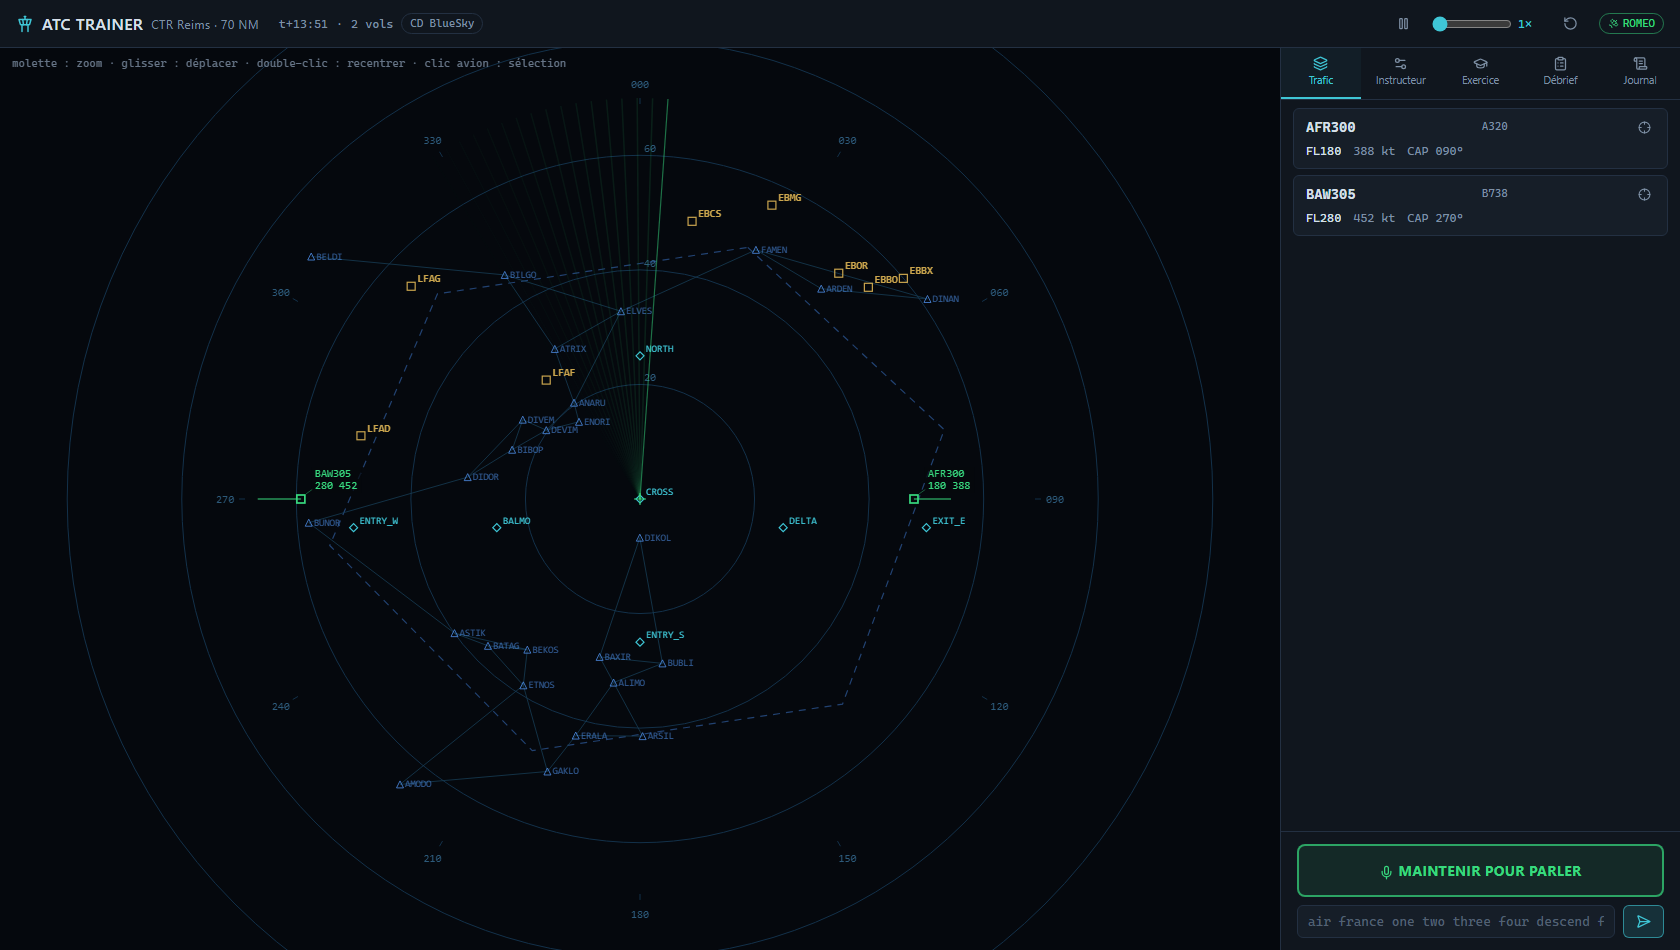
\includegraphics[width=0.92\textwidth]{figures/app_romeo.png}
\caption{Application en mode ROMEO : apres une clairance vocale, l'aeronef AFR300 est
etabli au FL180 et collationne dans sa voix clonee. La transcription de l'instruction
apparait sous le bouton \emph{push-to-talk}.}
\label{fig:romeo}
\end{figure}

\subsection{Resultats et mesures}

\begin{resbox}
\begin{itemize}
  \item \textbf{Latence de synthese} : 3,9~s par collationnement, facteur temps reel
  0,82 (XTTS sur CPU, n~=~3).
  \item \textbf{WER de re-transcription} de la voix synthetisee : 22 a 24~\%
  (mesure sur la boucle S6/S8).
  \item \textbf{Boucle vocale complete} rejouee et verifiee de bout en bout
  (2026-06-11).
  \item \textbf{Trois voix de reference} clonees, attribuees a des aeronefs distincts.
\end{itemize}
\end{resbox}

\noindent\textbf{Analyse.} La re-transcription de la voix synthetisee atteint un WER
de 22 a 24~\%, contre 6,7~\% pour une voix humaine reelle (validation de la
semaine~4). Cet ecart est attendu : la boucle voix-clonee~$\rightarrow$~Whisper
cumule les erreurs de deux modeles successifs (la synthese et la reconnaissance), et
la voix synthetique presente des caracteristiques hors du domaine d'entrainement du
module de reconnaissance. Ce taux confirme neanmoins que le collationnement reste
\emph{intelligible} et exploitable pour un retour radio dans un contexte
d'entrainement. La synthese reste par ailleurs stochastique : sur un meme texte, une
generation propre et une generation plus degradee ont ete observees. Avec un facteur
temps reel de l'ordre de 0,82 sur CPU, la synthese n'autorise pas un flux continu en
temps reel, mais reste compatible avec le rythme d'une frequence reelle (un echange
toutes les dizaines de secondes).

%=============================================================================
\section{Bilan et transition}
%=============================================================================

La semaine~6 complete la boucle de dialogue par un module de restitution vocale.
Le clonage \emph{zero-shot} XTTS-v2 genere a la volee une voix distincte par aeronef
sans entrainement par locuteur, et la degradation VHF reutilisee de la semaine~2
assure a la fois le realisme radio et la coherence de domaine avec le module de
reconnaissance. L'integration a ete validee de bout en bout : une clairance parlee
provoque la manoeuvre de l'aeronef dans BlueSky, suivie d'un collationnement
audible dans la voix clonee du pilote.

\medskip
\noindent\textbf{Prochaines etapes.} Les etapes suivantes visent a alimenter le LLM
par l'etat de trafic courant (requete situee), puis a consolider la mise en service
temps reel de la boucle complete et a mener une evaluation quantitative sur des
scenarios complets. Les limites identifiees cette semaine (variance de la synthese,
execution CPU non temps reel, WER de re-transcription accru) orientent ces travaux,
notamment vers une attenuation des cas de synthese degradee et une mesure
systematique de l'intelligibilite.

\vfill
\begin{center}
\small\color{atcblue}\rule{0.5\textwidth}{0.6pt}\\[4pt]
\textit{Rapport d'avancement, Semaine 6, Nicolas Marano}\\
\textit{Stage : copilote IA pour le controle aerien, URCA / supercalculateur ROMEO}
\end{center}

\end{document}
